\documentclass[fleqn]{article}
\usepackage[spanish,es-noshorthands]{babel}
\usepackage[utf8]{inputenc} 
\usepackage[papersize={5.5in,8.5in},total={4.5in,7.25in},centering]{geometry}
\usepackage{mathexam}
\usepackage{amsmath}
\usepackage{graphicx}
\usepackage{tikz,pgf}
\usetikzlibrary{arrows}
\usepackage{multicol}

\ExamClass{
\includegraphics[height=16pt]{Images/logo-sed.png} Aritmética $^{\circ}$}
\ExamName{``Introd. Fracciones''}
\ExamHead{
\includegraphics[height=16pt]{Images/logo-colegio.png} IEDAB}
\newcommand{\LineaNombre}{%
\par
\vspace{\baselineskip}
Nombre:\hrulefill \; Curso: \underline{\hspace*{48pt}} \; Fecha: \underline{\hspace*{2.5cm}} \relax
\par}
\let\ds\displaystyle

\begin{document}
\ExamInstrBox{
Respuesta sin justificar mediante procedimiento no será tenida en cuenta en la calificación. Escriba sus respuestas en el espacio indicado. Tiene 45 minutos para contestar esta prueba.}
\LineaNombre
\begin{enumerate}
 \item Descomponga los números compuestos siguientes, en sus factores primos y escriba el número como su producto. Ejm: $18=2\cdot 3^{2}$
 \begin{enumerate}
 \begin{multicols}{4}
  \item 48
  \item 96
  \item 60
  \item 150 
 \end{multicols}
 \end{enumerate}
 \item Identifique en las siguientes gráficas la fracción correspondiente a la región sombreada, escríbala y si se puede, simplifíquela.
 \begin{enumerate}
 \begin{multicols}{2}
\item \definecolor{zzttqq}{rgb}{0.6,0.2,0.}
\begin{tikzpicture}[line cap=round,line join=round,>=triangle 45,x=1.0cm,y=1.0cm]
\clip(-4.92,0.34) rectangle (-2.1,3.14);
\draw (-4.740281662206479,2.1827687752661227)-- (-2.36,1.34);
\draw (-2.59014083110324,2.5813843876330616)-- (-4.51014083110324,0.9413843876330616);
\draw(-3.5501408311032407,1.761384387633062) circle (1.26253712816693cm);
\draw (-3.78028166220648,3.0027687752661225)-- (-3.32,0.52);
\draw [shift={(-3.5501408311032407,1.761384387633062)},color=zzttqq,fill=zzttqq,fill opacity=0.6]  (0,0) --  plot[domain=-1.3874870416330785:2.801303163153312,variable=\t]({1.*1.2625371281669315*cos(\t r)+0.*1.2625371281669315*sin(\t r)},{0.*1.2625371281669315*cos(\t r)+1.*1.2625371281669315*sin(\t r)}) -- cycle ;
\end{tikzpicture}
 \item \definecolor{zzttqq}{rgb}{0.6,0.2,0.}
\begin{tikzpicture}[line cap=round,line join=round,>=triangle 45,x=1.0cm,y=1.0cm,scale=.4]
\clip(-4.94,-3.24) rectangle (5.6,4.);
\draw (0.32142135623730983,2.9758787847867993)-- (-2.3958787847868,-2.61857864376269);
\draw (-3.8344574285494897,1.5373001410241098)-- (1.76,-1.18);
\draw(-1.037228714274745,0.17865007051205492) circle (3.1097296496746387cm);
\draw (-2.0544574285494894,3.117300141024109)-- (-0.02,-2.76);
\draw (-3.9758787847867993,-0.8385786437626899)-- (1.9014213562373095,1.1958787847867993);
\draw [shift={(-1.037228714274745,0.17865007051205492)},color=zzttqq,fill=zzttqq,fill opacity=0.6]  (0,0) --  plot[domain=1.1186435857875154:5.045634402774757,variable=\t]({1.*3.1097296496746387*cos(\t r)+0.*3.1097296496746387*sin(\t r)},{0.*3.1097296496746387*cos(\t r)+1.*3.1097296496746387*sin(\t r)}) -- cycle ;
\end{tikzpicture}
  \end{multicols}
 \end{enumerate}
 \item Encuentre 10 fracciones equivalentes a cada una de las siguientes fracciones:
 \begin{enumerate}
 \item $\dfrac{2}{3}=\dfrac{4}{6}=$ \dots
 \item $\dfrac{1}{3}=$
 \item $\dfrac{5}{6}=$
 \item $\dfrac{7}{8}=$
  \item $\dfrac{5}{8}=$
 \end{enumerate}
  \item A continuación encuentras dos hexágonos regulares (congruentes y semejantes). Tomando cada polígono como una unidad.
\begin{center}
 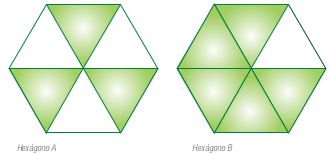
\includegraphics[scale=.5]{Images/hexagonos.png} 
 \end{center} 
 Responde lo siguiente:
 \begin{enumerate}
 \item Cada unidad está dividida en \underline{\hspace*{20pt}} partes
iguales.
 \item El hexágono A tiene \underline{\hspace*{20pt}} partes sombreadas.
 \item El hexágono B tiene \underline{\hspace*{20pt}} partes sombreadas.
 \item Verifica si el total de partes sombreadas entre los dos hexágonos es mayor que una unidad. Explica por qué y de ser así, exprésalo como un
número mixto.\noanswer[1in]
 \end{enumerate}
 \item Luisita bajó 18 naranjas del cultivo que tiene en su finca y $\frac{1}{3}$ de ellas se lo dio Natalia. ¿Cuántas naranjas dejó para ella?\noanswer

 \end{enumerate}

\end{document}
